\documentclass[10pt]{beamer}
\usetheme{Madrid} % Bạn có thể đổi sang theme khác như Warsaw, Frankfurt...
\usecolortheme{default}

% ----- ENCODING & LANGUAGE -----
\usepackage[utf8]{inputenc}
\usepackage[T5]{fontenc}
\usepackage[english,vietnamese]{babel}

% ----- GRAPHICS & CODE -----
\usepackage{graphicx}
\usepackage{listings}
\usepackage{xcolor}

% ---- Tái sử dụng màu và style từ mystyle.sty ----
\definecolor{keywordcolor}{rgb}{0.1,0.1,0.6}
\definecolor{commentcolor}{rgb}{0.0,0.5,0.0}
\definecolor{stringcolor}{rgb}{0.58,0,0.82}
\definecolor{bgcolor}{rgb}{0.95,0.95,0.95}

\lstdefinestyle{verilog-style}{
	language=Verilog,
	backgroundcolor=\color{bgcolor},
	keywordstyle=\color{keywordcolor}\bfseries,
	commentstyle=\color{commentcolor}\itshape,
	stringstyle=\color{stringcolor},
	basicstyle=\ttfamily\scriptsize, % Chỉnh font nhỏ lại cho vừa slide
	numbers=left,
	numberstyle=\tiny,
	stepnumber=1,
	numbersep=5pt,
	tabsize=2,
	showstringspaces=false,
	breaklines=true,
	frame=single
}

% ----- THÔNG TIN TRANG BÌA -----
\title[RISC-V Single-Cycle]{Design and Implementation of a \\ 32-bit Single-Cycle RISC-V Processor}
\author{NGUYEN DUY TUYEN}
\institute{GROUP 5}
\date{\today}

\begin{document}
	
	% Slide tiêu đề
	\begin{frame}
		\titlepage
	\end{frame}
	
	% Slide mục lục
	\begin{frame}{Nội dung trình bày}
		\tableofcontents
	\end{frame}
	
	% Nạp nội dung slide
	\section{Giới thiệu tổng quan}
\section{Giới thiệu tổng quan}
\begin{frame}{Giới thiệu tổng quan}
	\begin{columns}[T]
		\begin{column}{0.35\textwidth}
			\footnotesize
			\textbf{Nội dung đồ án:}
			\begin{itemize}
				\item Thiết kế và triển khai bộ xử lý RISC-V 32-bit Single-Cycle (RV32I).
				\item Tích hợp đầy đủ các khối chức năng: ALU, BRC, Regfile, ImmGen, Control Unit.
				\item Giao tiếp phần cứng ngoại vi thông qua khối Load-Store Unit (LSU) sử dụng kỹ thuật \textbf{Memory-Mapped I/O}.
				\item Tổng hợp toàn bộ hệ thống và thực thi các ứng dụng viết bằng Assembly trên kit FPGA DE-2/DE2-115.
			\end{itemize}
		\end{column}
		
		\begin{column}{0.65\textwidth}
			\begin{figure}
				\centering
				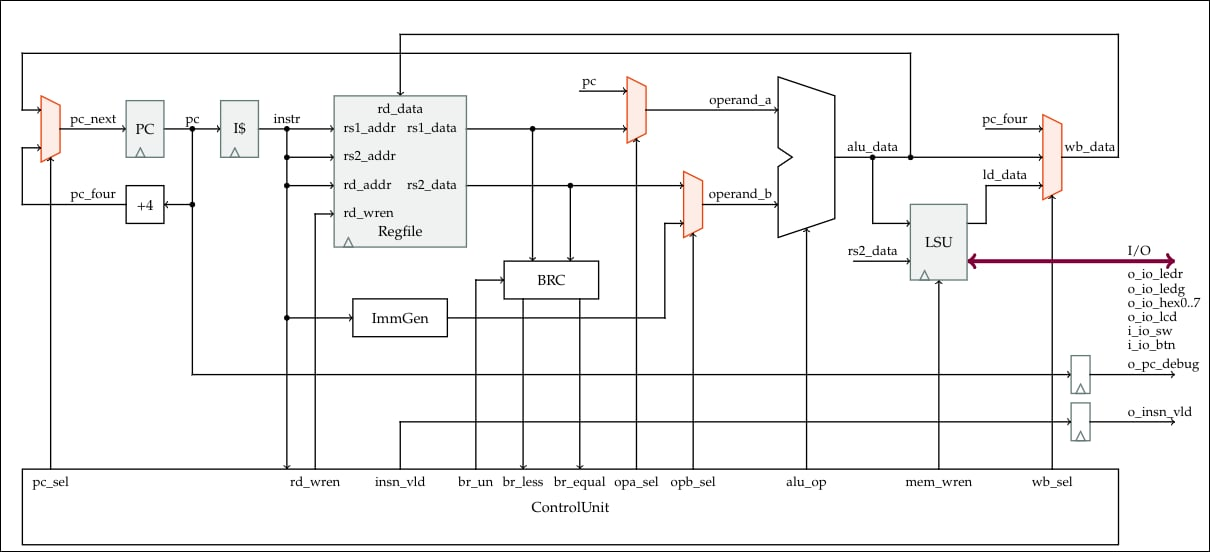
\includegraphics[width=1.0\linewidth]{figures_tech/single.jpg}
				\caption{\footnotesize Sơ đồ kiến trúc Single Cycle Processor}
			\end{figure}
		\end{column}
	\end{columns}
\end{frame}

\section{Chiến lược thiết kế (Design Strategy)}
% ==========================================
% SLIDE: ALU (Hình ảnh lớn hơn)
% ==========================================
\begin{frame}{Khối Arithmetic Logic Unit (ALU)}
	\begin{columns}[T]
		\begin{column}{0.35\textwidth} % Thu hẹp cột văn bản
			\footnotesize
			\textbf{Chức năng \& Tối ưu:}
			\begin{itemize}
				\item Xử lý các phép toán số học và logic giữa \texttt{i\_a} và \texttt{i\_b}.
				\item \textbf{Loại bỏ toán tử built-in:} Tuân thủ đặc tả tổng hợp phần cứng.
				\item \textbf{Gộp phép toán:} Tái sử dụng \texttt{cla\_adder\_top} cho phép cộng, trừ và so sánh.
				\begin{itemize}
					\item \textit{Có dấu (SLT):} \texttt{Sum[31]} XOR \texttt{overflow}.
					\item \textit{Không dấu (SLTU):} Đảo của cờ \texttt{C\_out}.
				\end{itemize}
				\item \textbf{Dịch bit (Shift):} Dùng module chuyên biệt \texttt{shift\_left/right}.
			\end{itemize}
		\end{column}
		
		\begin{column}{0.65\textwidth} % Mở rộng cột hình ảnh
			\begin{figure}
				\centering
				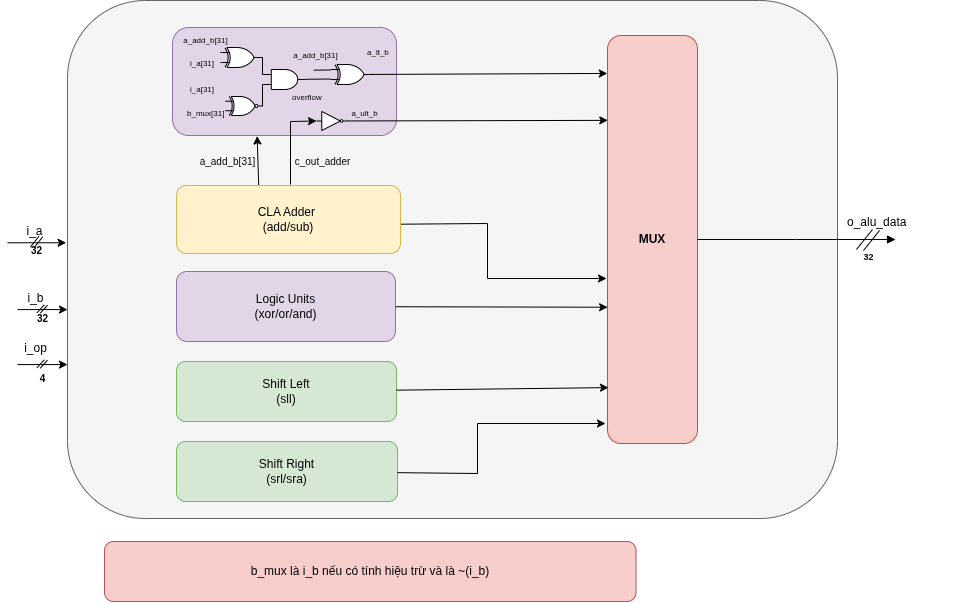
\includegraphics[width=1.0\linewidth]{figures_tech/alu111.png}
				\caption{\footnotesize Sơ đồ khối ALU Datapath}
			\end{figure}
		\end{column}
	\end{columns}
\end{frame}

% ==========================================
% SLIDE: BRC (Hình ảnh lớn hơn)
% ==========================================
\begin{frame}{Khối Branch Comparison Unit (BRC)}
	\begin{columns}[T]
		\begin{column}{0.35\textwidth} % Thu hẹp cột văn bản
			\footnotesize
			\textbf{Đặc điểm thiết kế:}
			\begin{itemize}
				\item Đánh giá điều kiện rẽ nhánh giữa \texttt{rs1} và \texttt{rs2}.
				\item Cấp phát module \texttt{cla\_adder\_top} cho phép trừ phần cứng (không dùng toán tử so sánh built-in).
				\item \textbf{o\_equal:} Áp dụng reduction NOR trên kết quả \texttt{a\_sub\_b}.
				\item \textbf{Xử lý linh hoạt:} Multiplexer chọn kết quả dựa trên tín hiệu \texttt{i\_br\_un}.
			\end{itemize}
		\end{column}
		
		\begin{column}{0.65\textwidth} % Mở rộng cột hình ảnh
			\begin{figure}
				\centering
				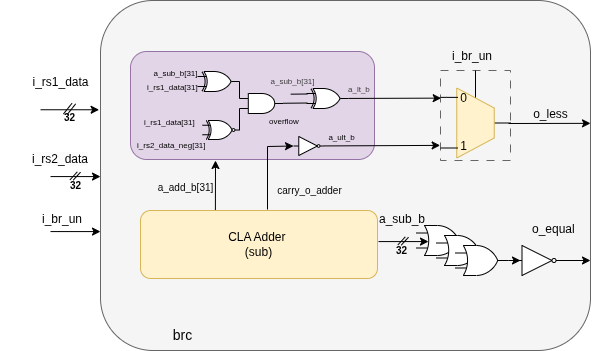
\includegraphics[width=1.0\linewidth]{figures_tech/brc111.png}
				\caption{\footnotesize Sơ đồ khối Branch Comparison}
			\end{figure}
		\end{column}
	\end{columns}
\end{frame}
% ==========================================
% SLIDE: Register File (Tối ưu hình ảnh)
% ==========================================
\begin{frame}{Tập thanh ghi (Register File)}
	\begin{columns}[T]
		\begin{column}{0.35\textwidth}
			\footnotesize
			\textbf{Cấu trúc hệ thống:}
			\begin{itemize}
				\item Gồm 32 thanh ghi 32-bit (từ \texttt{x0} đến \texttt{x31}) phục vụ lưu trữ toán hạng.
				\item \textbf{Cơ chế đọc:} Hỗ trợ hai cổng đọc độc lập, truy xuất đồng thời \texttt{rs1}, \texttt{rs2} (đọc bất đồng bộ).
				\item \textbf{Cơ chế ghi:} Ghi vào \texttt{rd} đồng bộ theo sườn lên xung nhịp khi \texttt{i\_reg\_wen} được kích hoạt.
			\end{itemize}
			
			\vspace{0.1cm}
			\textbf{Đặc điểm kỹ thuật:}
			\begin{itemize}
				\item \textbf{Thanh ghi x0:} Được nối cứng xuống mức logic 0. Mọi thao tác ghi đều bị bỏ qua và đọc luôn trả về giá trị 0.
				\item Đảm bảo tính toàn vẹn dữ liệu nhờ sự kết hợp giữa đọc tổ hợp và ghi tuần tự.
			\end{itemize}
		\end{column}
		
		\begin{column}{0.65\textwidth}
			\begin{figure}
				\centering
				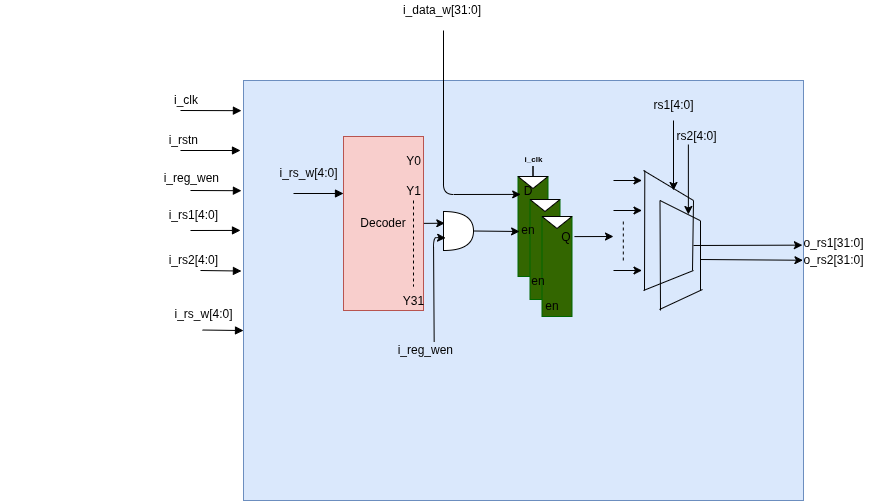
\includegraphics[width=1.0\linewidth]{figures_tech/reg_file.png}
				\caption{\footnotesize Kiến trúc chi tiết của khối Regfile}
			\end{figure}
		\end{column}
	\end{columns}
\end{frame}
% ==========================================
% SLIDE 1: LSU - CƠ CHẾ TRUY XUẤT (Hình ảnh lớn)
% ==========================================
\begin{frame}{Khối Load-Store Unit (LSU) - Truy xuất dữ liệu}
	\begin{columns}[T]
		\begin{column}{0.35\textwidth}
			\footnotesize
			\textbf{Chức năng chính:}
			\begin{itemize}
				\item Cầu nối dữ liệu giữa CPU và hệ thống ngoại vi (\textbf{Memory-Mapped I/O}).
			\end{itemize}
			
			\vspace{0.1cm}
			\textbf{Xử lý lệnh Store:}
			\begin{itemize}
				\item Tạo mask 4-bit (\texttt{i\_bmask}) từ 2 bit địa chỉ thấp.
				\item Ghi chọn lọc theo Byte, Half-word hoặc Word vào bộ nhớ.
			\end{itemize}
			
			\vspace{0.1cm}
			\textbf{Xử lý lệnh Load:}
			\begin{itemize}
				\item Tự động căn lề phải dữ liệu.
				\item \textbf{Mở rộng bit:} Sign-Extension (\texttt{LB, LH}) hoặc Zero-Extension (\texttt{LBU, LHU}) dựa trên \texttt{i\_funct3}.
			\end{itemize}
		\end{column}
		
		\begin{column}{0.65\textwidth}
			\begin{figure}
				\centering
				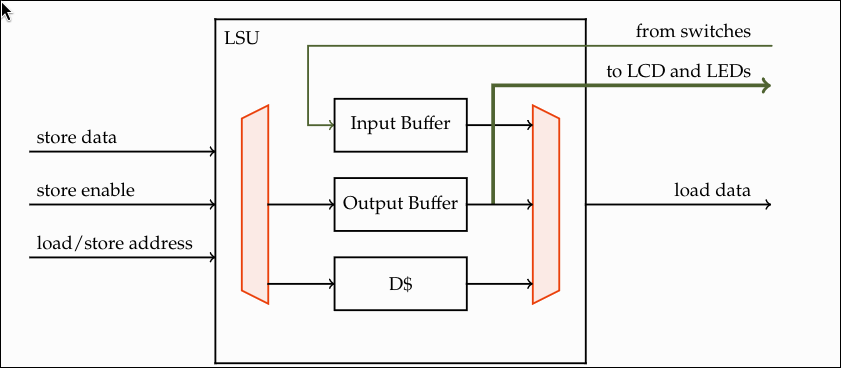
\includegraphics[width=1.0\linewidth]{figures_tech/lsu.png}
				\caption{\footnotesize Sơ đồ khối chức năng của LSU}
			\end{figure}
		\end{column}
	\end{columns}
\end{frame}

% ==========================================
% SLIDE 2: LSU - Ánh xạ bộ nhớ (Memory Mapping)
% ==========================================
\begin{frame}{LSU - Giải mã địa chỉ \& Ngoại vi}
	\begin{columns}[T]
		% --- CỘT TRÁI: TEXT GIẢI THÍCH ---
		\begin{column}{0.4\textwidth}
			\footnotesize
			\textbf{Giải mã địa chỉ:}
			\begin{itemize}
				\item Sử dụng 20 bit cao (\texttt{addr[31:12]}) để phân vùng thiết bị.
				\item Kích hoạt các tín hiệu Chip Select tương ứng cho RAM hoặc I/O.
			\end{itemize}
			
			\vspace{0.2cm}
			\textbf{Giao tiếp ngoại vi:}
			\begin{itemize}
				\item Tích hợp các module Buffer để đồng bộ hóa tín hiệu từ vi xử lý với chân vật lý trên kit FPGA DE2.
				\item Đảm bảo đáp ứng thời gian (timing) khi truy xuất.
			\end{itemize}
		\end{column}
		
		% --- CỘT PHẢI: BẢNG MEMORY MAPPING ---
		\begin{column}{0.6\textwidth}
			\vspace{-0.1cm} % Kéo bảng lên một chút cho cân đối
			\begin{table}[]
				\centering
				\renewcommand{\arraystretch}{1.2}
				% Ép kích thước bảng vừa khít chiều rộng cột để không bị tràn
				\resizebox{\linewidth}{!}{%
					\begin{tabular}{|l|l|l|}
						\hline
						\textbf{Base address} & \textbf{Top address} & \textbf{Mapping} \\ \hline
						\texttt{0x1001\_1000} & \texttt{0xFFFF\_FFFF} & (Reserved) \\ \hline
						\texttt{0x1001\_0000} & \texttt{0x1001\_0FFF} & Switches \textcolor{red}{\textit{(required)}} \\ \hline
						\texttt{0x1000\_5000} & \texttt{0x1000\_FFFF} & (Reserved) \\ \hline
						\texttt{0x1000\_4000} & \texttt{0x1000\_4FFF} & LCD Control Registers \\ \hline
						\texttt{0x1000\_3000} & \texttt{0x1000\_3FFF} & Seven-segment LEDs 7-4 \\ \hline
						\texttt{0x1000\_2000} & \texttt{0x1000\_2FFF} & Seven-segment LEDs 3-0 \\ \hline
						\texttt{0x1000\_1000} & \texttt{0x1000\_1FFF} & Green LEDs \textcolor{red}{\textit{(required)}} \\ \hline
						\texttt{0x1000\_0000} & \texttt{0x1000\_0FFF} & Red LEDs \textcolor{red}{\textit{(required)}} \\ \hline
						\texttt{0x0000\_0800} & \texttt{0x0FFF\_FFFF} & (Reserved) \\ \hline
						\texttt{0x0000\_0000} & \texttt{0x0000\_07FF} & Memory (2KiB) \textcolor{red}{\textit{(required)}} \\ \hline
					\end{tabular}%
				}
			\end{table}
		\end{column}
	\end{columns}
\end{frame}
\begin{frame}{Khối Điều Khiển (Control Unit)}
	\begin{columns}
		\begin{column}{0.5\textwidth}
			\begin{itemize}
				\item Giải mã lệnh 32-bit từ Instruction Memory để tạo tín hiệu điều khiển cho Datapath.
				\item Xác định loại lệnh (I, S, B, U, J) để Immediate Generator trích xuất giá trị.
				\item Điều khiển bộ dồn kênh (Multiplexer) chọn nguồn dữ liệu cho PC, ALU và Regfile.
			\end{itemize}
		\end{column}
		\begin{column}{0.5\textwidth}
			\begin{figure}
				\centering
				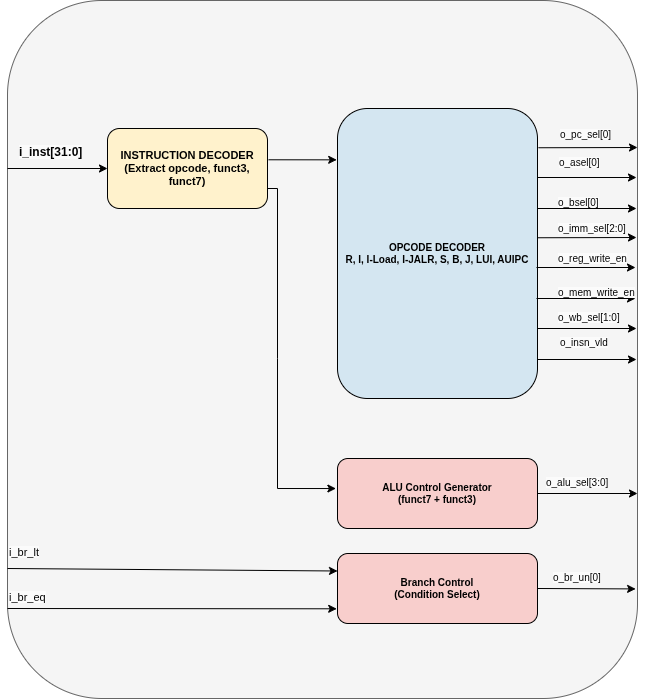
\includegraphics[width=1.0\linewidth]{figures_tech/ctrl.png}
				\caption{Control Logic}
			\end{figure}
		\end{column}
	\end{columns}
\end{frame}
\section{Triển khai trên FPGA (Hardware Implementation)}

% ==========================================
% SLIDE 1: THUẬT TOÁN & CƠ CHẾ
% ==========================================
\begin{frame}{Ứng dụng 1: Điều khiển LED qua Switch (Cơ chế \& Thuật toán)}
	\begin{columns}[T]
		\begin{column}{0.6\textwidth}
			\small
			\textbf{Cơ chế hoạt động:}
			\begin{itemize}
				\item Luồng dữ liệu trực tiếp từ Switch sang Red LED qua kỹ thuật \textbf{Memory-Mapped I/O}.
			\end{itemize}
			
			\vspace{0.1cm}
			\textbf{Quy trình xử lý:}
			\begin{enumerate}
				\item \textbf{Khởi tạo:} Dùng lệnh \texttt{lui} nạp địa chỉ Switch (\texttt{0x10010000}) và LEDR (\texttt{0x10000000}).
				\item \textbf{Vòng lặp Polling:} Thực hiện lệnh \texttt{lw} liên tục để đọc trạng thái logic (On/Off) của các công tắc vào thanh ghi tạm.
				\item \textbf{Cập nhật:} Lệnh \texttt{sw} ghi giá trị vào địa chỉ LEDR để điều khiển đèn.
				\item \textbf{Duy trì:} Lệnh \texttt{jal} quay lại để cập nhật trạng thái liên tục.
			\end{enumerate}
		\end{column}
		
		\begin{column}{0.3\textwidth}
			\begin{figure}
				\centering
				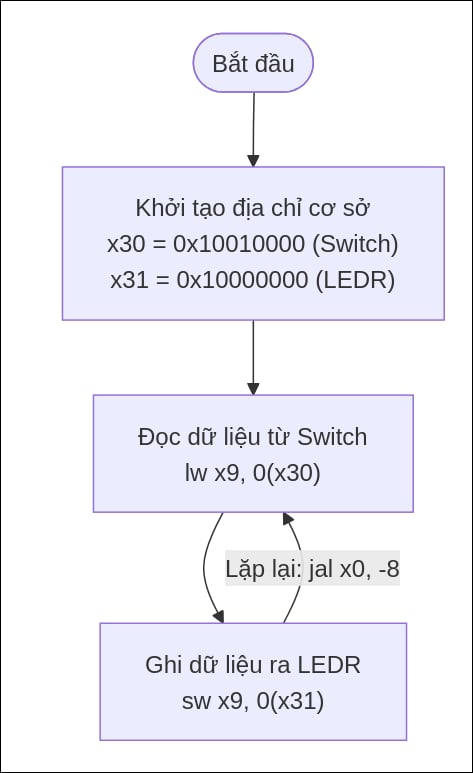
\includegraphics[width=\linewidth]{figures_tech/sw_ledr.jpg}
				\caption{\footnotesize Lưu đồ thuật toán MMIO}
			\end{figure}
		\end{column}
	\end{columns}
\end{frame}

% ==========================================
% SLIDE 2: THỰC THI TRÊN KIT & GIẢI THÍCH
% ==========================================
\begin{frame}{Ứng dụng 1: Kết quả thực hiện trên Kit DE2}
	\begin{columns}[T]
		\begin{column}{0.45\textwidth}
			\begin{figure}
				\centering
				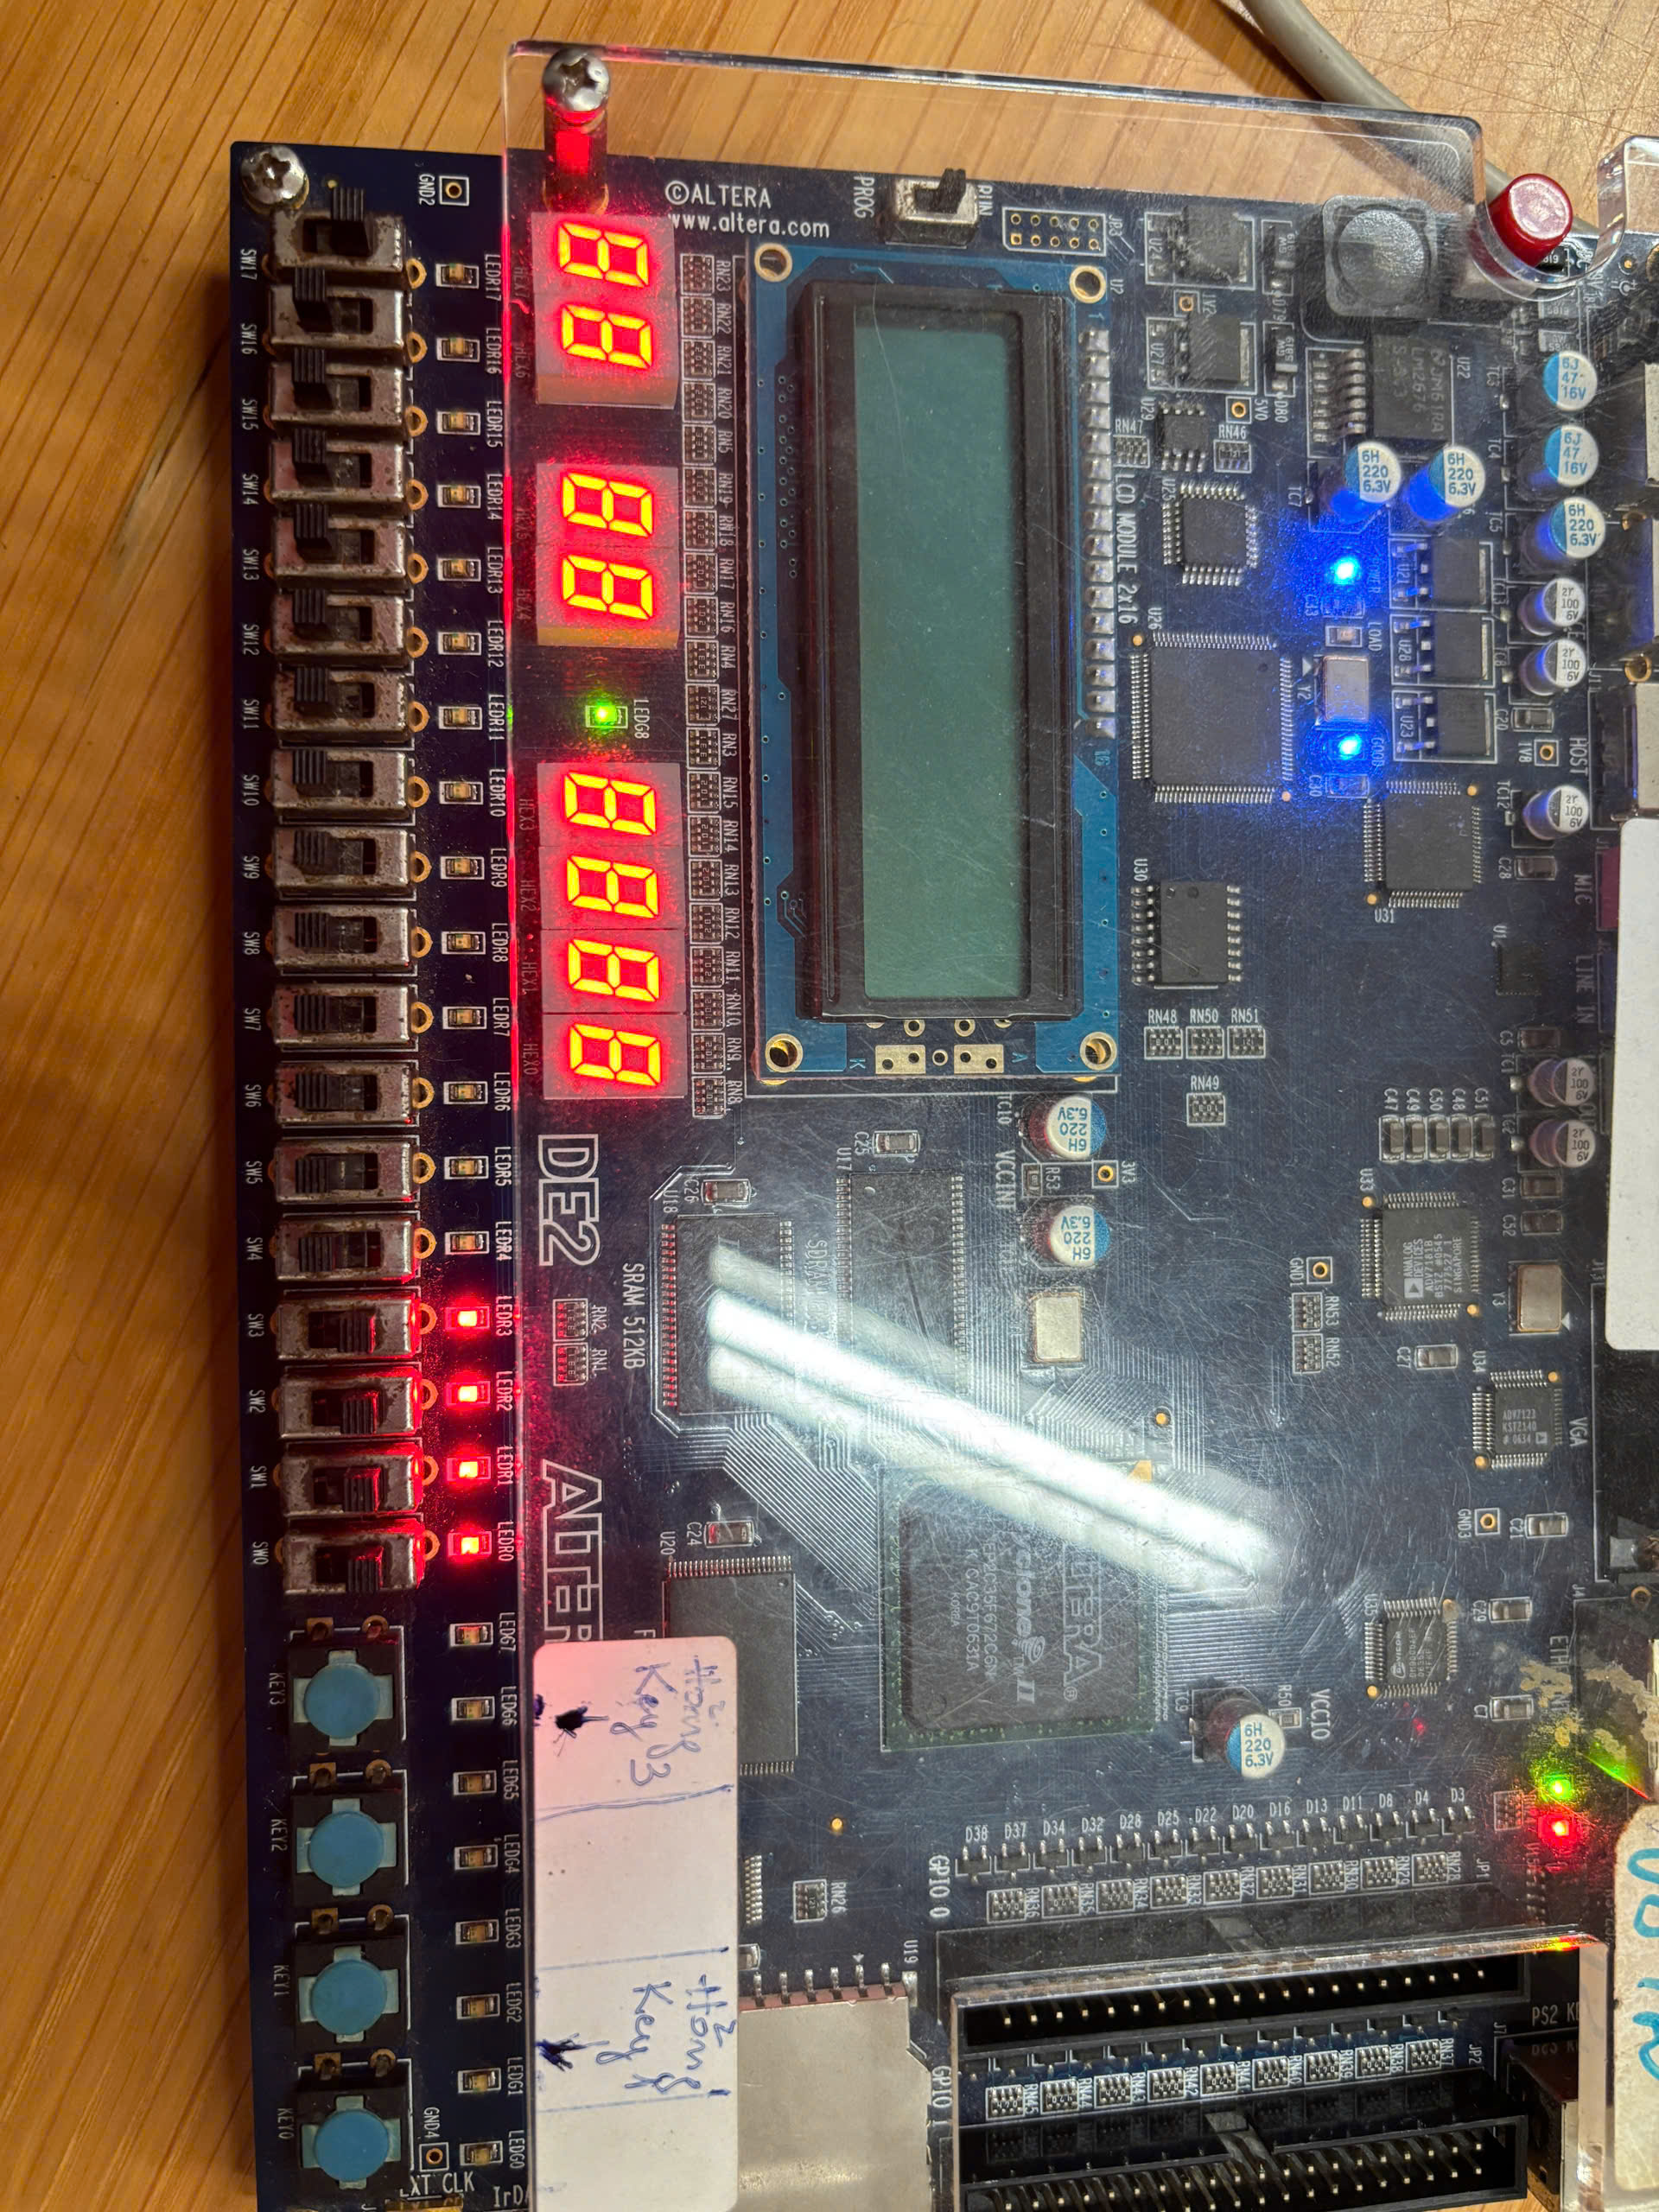
\includegraphics[width=\linewidth]{figures_tech/sw_2_ledr.jpg}
				\caption{\footnotesize LED phản hồi thực tế trên Kit}
			\end{figure}
		\end{column}
		
		\begin{column}{0.55\textwidth}
			\footnotesize
			\textbf{Giải thích và Đánh giá:}
			\begin{itemize}
				\item \textbf{Đáp ứng thời gian thực:} Kiến trúc Single-Cycle cho phép thực hiện đọc-ghi trong một chu kỳ, giúp lấy mẫu trạng thái Switch với tần số cao và độ trễ cực thấp.
				\item \textbf{Tương tác vật lý:} Các đèn LED đỏ phản hồi chính xác và đồng bộ theo thời gian thực ngay khi người dùng thay đổi vị trí các công tắc gạt.
				\item \textbf{Độ tin cậy:} Hệ thống hoạt động ổn định, chứng minh khối LSU và phần giải mã địa chỉ ngoại vi được thiết kế chính xác theo đặc tả yêu cầu.
			\end{itemize}
		\end{column}
	\end{columns}
\end{frame}

% ==========================================
% SLIDE 1: THUẬT TOÁN XỬ LÝ DỮ LIỆU (Đã fix tràn hình)
% ==========================================
\begin{frame}{Ứng dụng 2: Hiển thị giá trị Switch lên HEX (Thuật toán)}
	\begin{columns}[T]
		\begin{column}{0.3\textwidth} % Thu nhỏ cột chữ để dành chỗ cho hình
			\footnotesize
			\textbf{Quy trình xử lý dữ liệu:}
			\begin{itemize}
				\item \textbf{Bước 1 - Masking:} Dùng mặt nạ 13-bit (\texttt{0x1FFF}) để lọc dữ liệu từ Switch, giới hạn tối đa 8191.
				\item \textbf{Bước 2 - Tách số:} 
				\begin{itemize}
					\item Dùng hàm \texttt{DIV10\_MOD10} chia lấy dư liên tiếp cho 10.
					\item Tách thành 6 chữ số thập phân riêng biệt.
				\end{itemize}
				\item \textbf{Bước 3 - Giải mã:} 
				\begin{itemize}
					\item Gọi hàm \texttt{HEX\_DECODE} tra bảng mã (Look-up Table).
					\item Chuyển đổi sang mã điều khiển (Ví dụ: \texttt{0x40} cho số '0').
				\end{itemize}
			\end{itemize}
		\end{column}
		
		\begin{column}{0.7\textwidth} % Mở rộng cột hình
			\begin{figure}
				\centering
				% Giới hạn cả chiều rộng và chiều cao để không bị tràn dọc hoặc ngang
				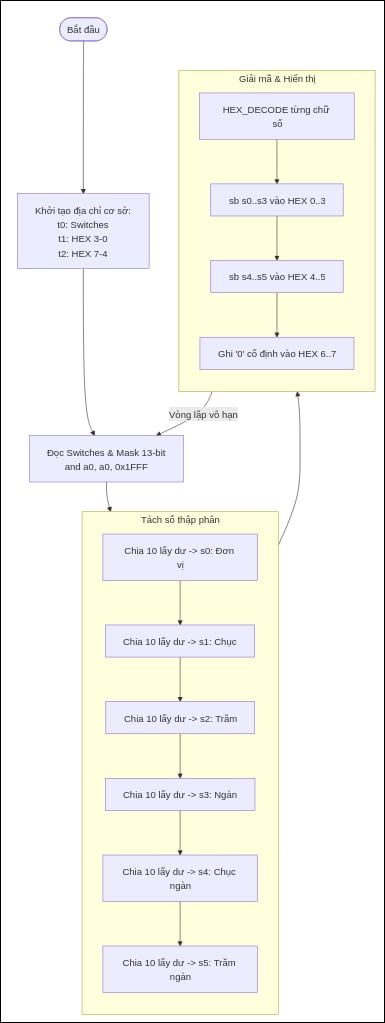
\includegraphics[width=\linewidth, height=0.75\textheight, keepaspectratio]{figures_tech/swhex.jpg}
				\caption{\footnotesize Lưu đồ thuật toán xử lý dữ liệu}
			\end{figure}
		\end{column}
	\end{columns}
\end{frame}

% ==========================================
% SLIDE 2: THỰC THI TRÊN KIT & KẾT QUẢ
% ==========================================
\begin{frame}{Ứng dụng 2: Kết quả thực hiện trên Kit DE2}
	\begin{columns}[T]
		\begin{column}{0.5\textwidth}
			\begin{figure}
				\centering
				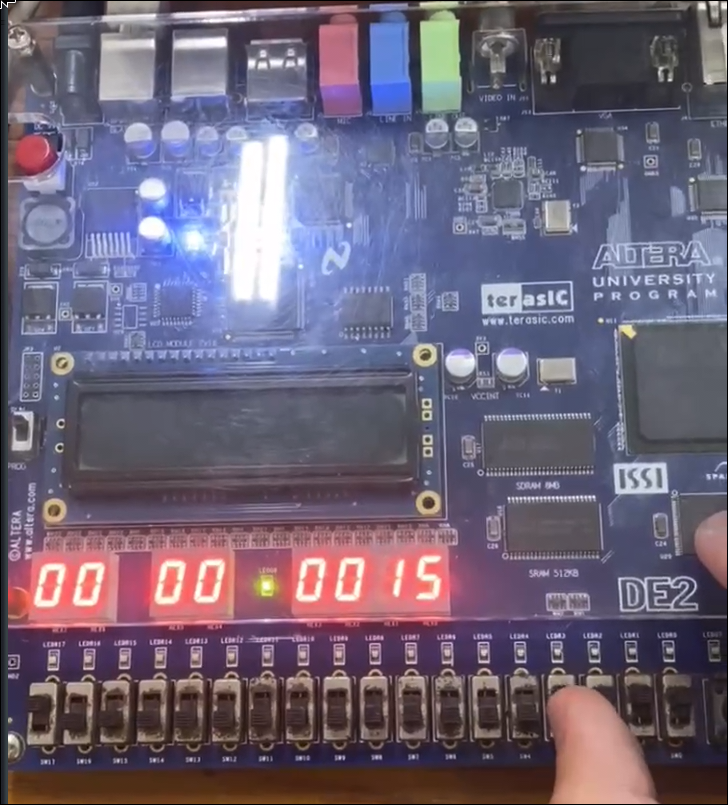
\includegraphics[width=\linewidth]{figures_tech/SW_to_HEX.png}
				\caption{\footnotesize Hiển thị thực tế số 15 (Switch = 1111)}
			\end{figure}
		\end{column}
		
		\begin{column}{0.5\textwidth}
			\footnotesize
			\textbf{Đánh giá kết quả thực nghiệm:}
			\begin{itemize}
				\item \textbf{Độ chính xác:} Dữ liệu nhị phân từ Switch được chuyển đổi sang hệ thập phân và hiển thị chính xác trên cụm HEX.
				\item \textbf{Địa chỉ I/O:} 
				\begin{itemize}
					\item 4 chữ số thấp xuất ra HEX 3-0 (\texttt{0x10002000}).
					\item 2 chữ số cao xuất ra HEX 5-4 (\texttt{0x10003000}).
				\end{itemize}
				\item \textbf{Đồng nhất hiển thị:} Hai LED cao nhất (HEX 7-6) được thiết lập mã \texttt{0x40} (số 0) để duy trì đủ 8 chữ số trên board.
				\item \textbf{Hiệu năng:} Phản hồi tức thời với thao tác gạt Switch nhờ tần số xử lý của kiến trúc Single-Cycle.
			\end{itemize}
		\end{column}
	\end{columns}
\end{frame}
% ==========================================
% SLIDE 1: THUẬT TOÁN STOPWATCH (Đã tối ưu hình lớn)
% ==========================================
\begin{frame}{Ứng dụng 3: Đồng hồ bấm giờ (Stopwatch)}
	\begin{columns}[T]
		\begin{column}{0.3\textwidth}
			\footnotesize
			\textbf{Cơ chế hoạt động:}
			\begin{itemize}
				\item \textbf{Đếm Ripple Carry:} Sử dụng 4 thanh ghi (\texttt{x12}-\texttt{x15}) lưu chữ số thập phân. Tự động tràn và reset khi đạt ngưỡng 10.
				\item \textbf{Tạm dừng (Pause):} Đọc trạng thái \texttt{SW0}. Nếu bật, CPU nhảy qua khối tăng giá trị để giữ nguyên thời gian.
				\item \textbf{Độ trễ (Delay):} Dùng hàm \texttt{DELAY\_n\_100ms} tạo khoảng nghỉ 0.5s giữa các lần đếm.
			\end{itemize}
		\end{column}
		
		\begin{column}{0.7\textwidth}
			\begin{figure}
				\centering
				% Giới hạn chiều cao 75% slide để không đẩy caption ra ngoài
				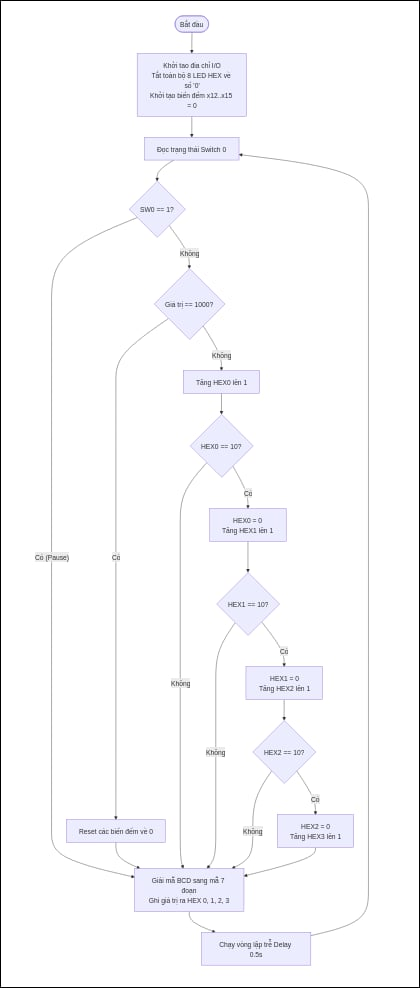
\includegraphics[width=\linewidth, height=0.75\textheight, keepaspectratio]{figures_tech/stw.jpg}
				\caption{\footnotesize Lưu đồ thuật toán đếm Stopwatch}
			\end{figure}
		\end{column}
	\end{columns}
\end{frame}

% ==========================================
% SLIDE 2: KẾT QUẢ THỰC NGHIỆM (Đã tối ưu hình lớn)
% ==========================================
\begin{frame}{Ứng dụng 3: Kết quả thực hiện trên Kit DE2}
	\begin{columns}[T]
		\begin{column}{0.3\textwidth}
			\footnotesize
			\textbf{Phân tích thực nghiệm:}
			\begin{itemize}
				\item \textbf{Tính chính xác:} Chuyển đổi BCD và giải mã HEX hiển thị khớp với biến đếm nội bộ.
				\item \textbf{Điều khiển:} Tính năng Pause phản hồi tức thời theo công tắc gạt \texttt{SW0} vật lý.
				\item \textbf{Hiển thị:} Thời gian hiển thị rõ nét trên 1 LED 7-đoạn đầu của cụm HEX 3-0.
				\item \textbf{Giới hạn:} Bộ đếm reset về 0 chính xác khi đạt mốc giới hạn thiết lập (1000).
			\end{itemize}
		\end{column}
		
		\begin{column}{0.7\textwidth}
			\begin{figure}
				\centering
				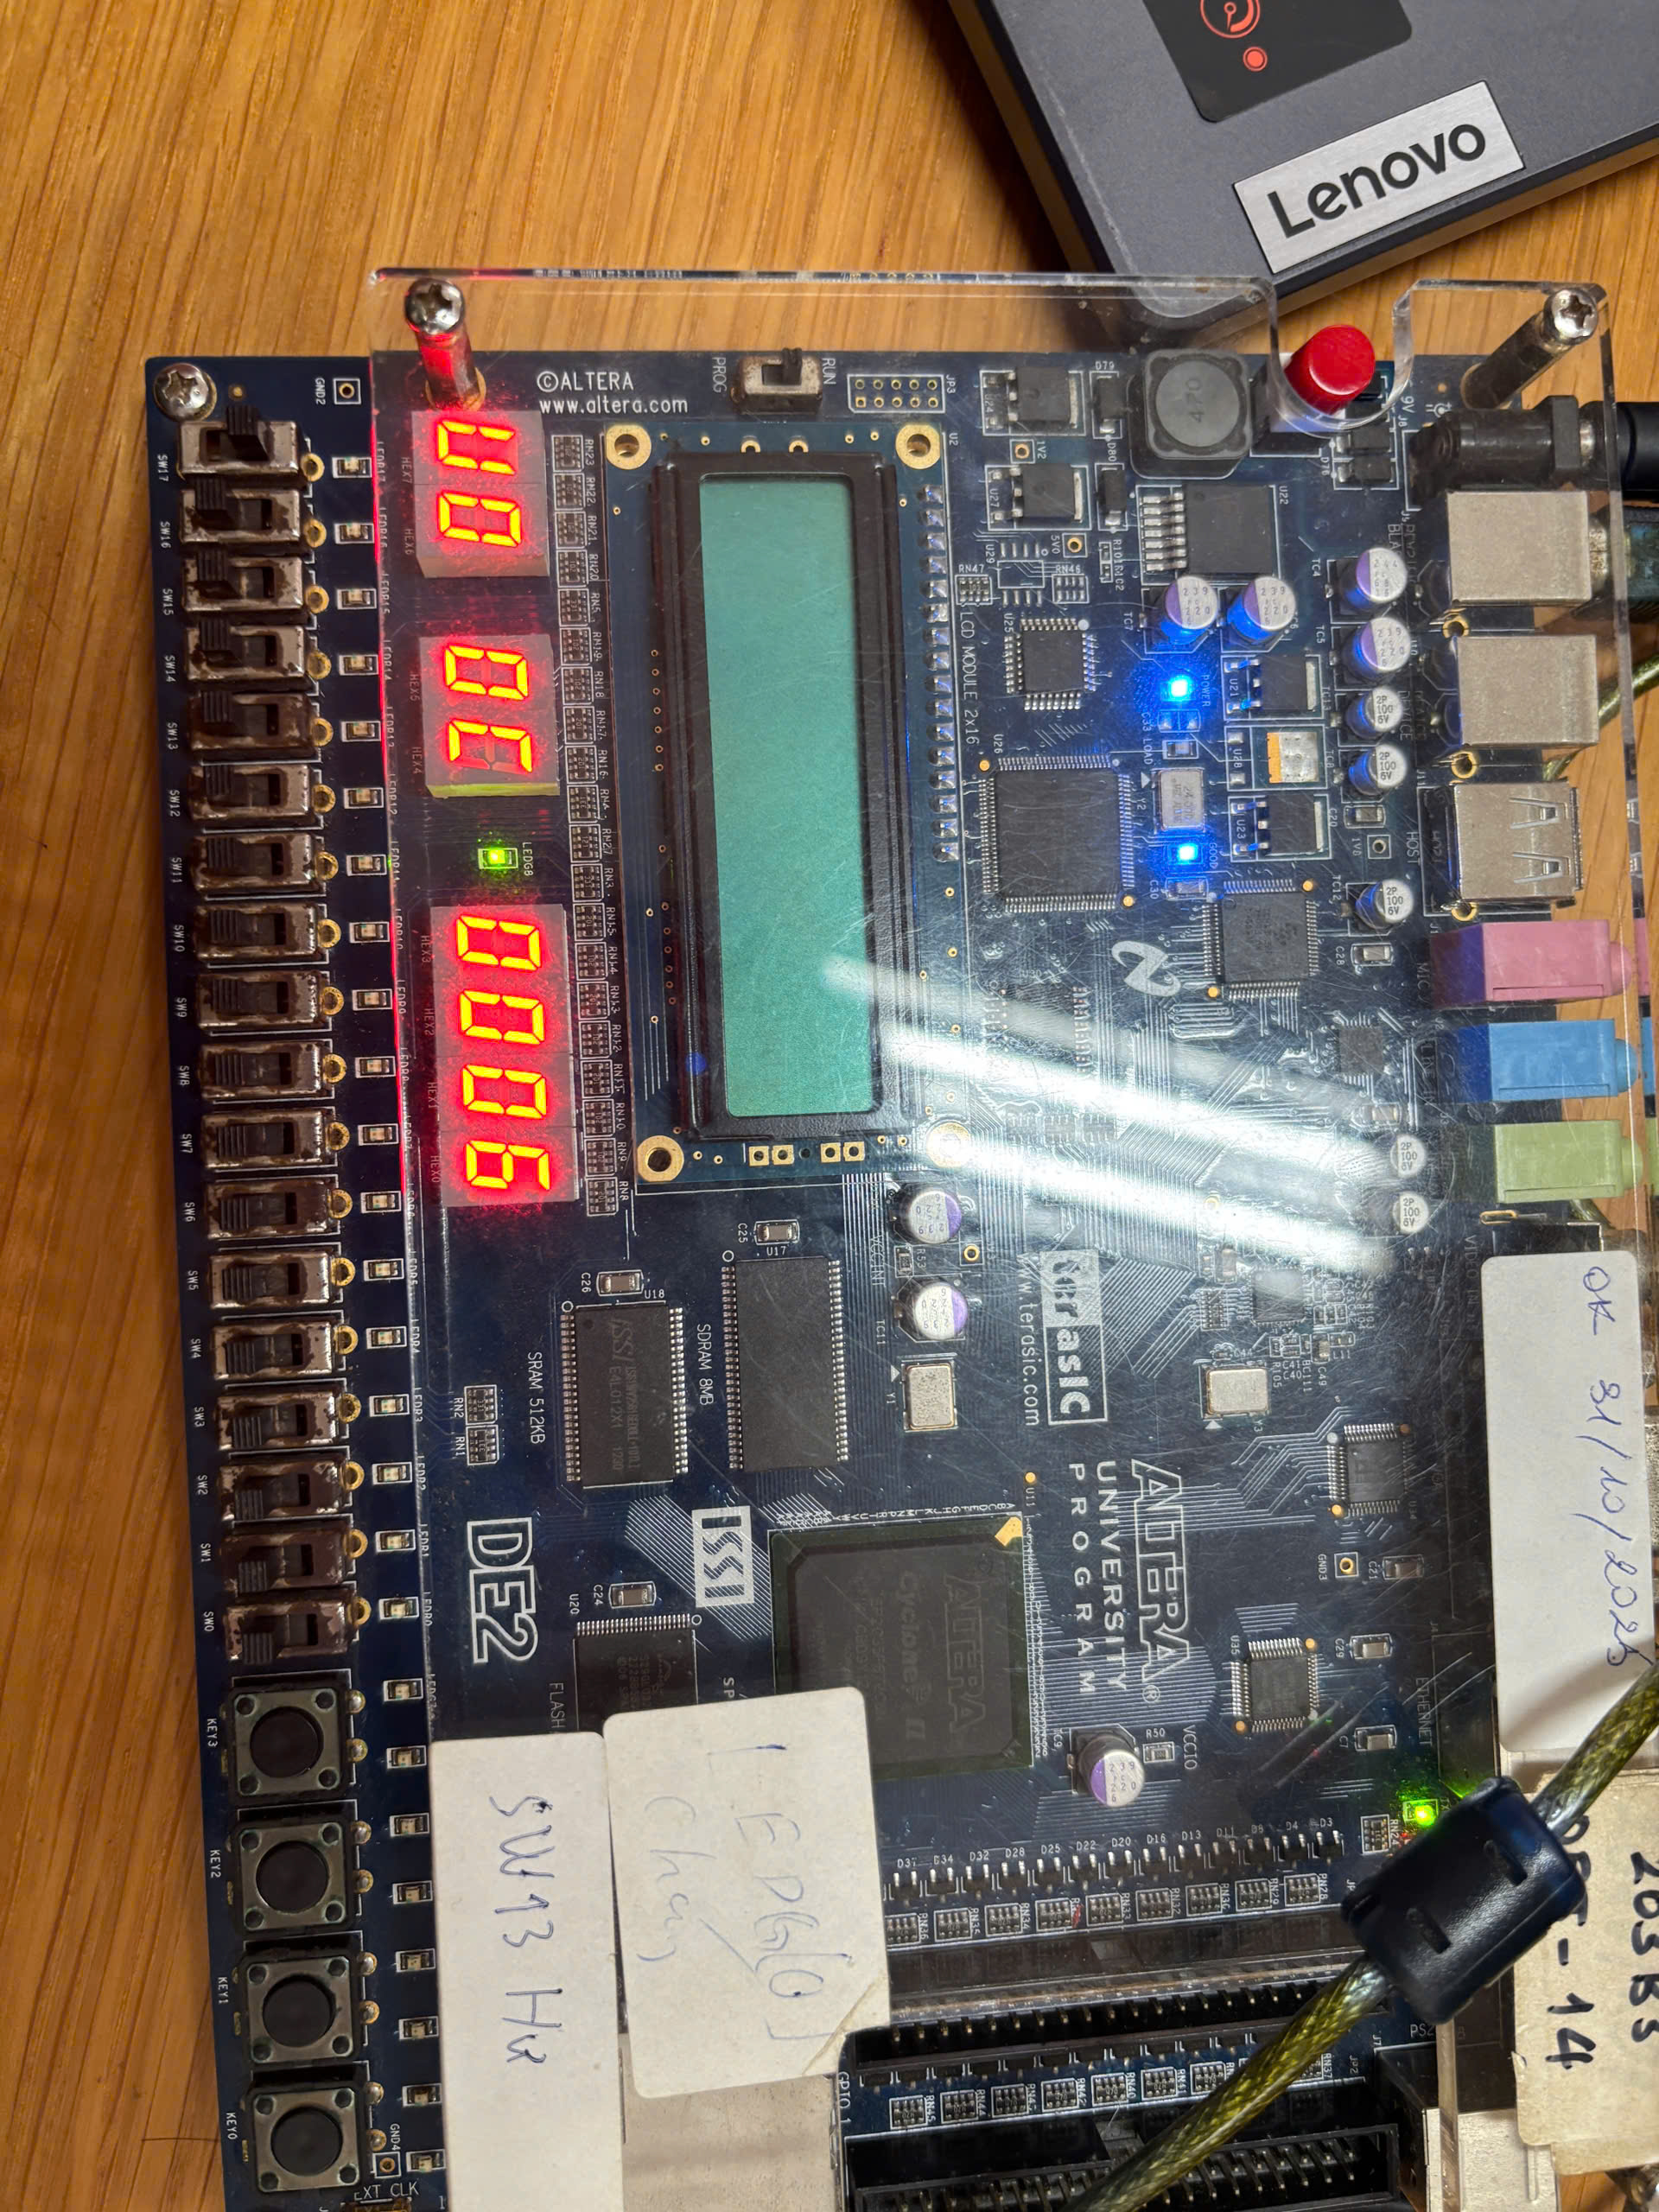
\includegraphics[width=\linewidth, height=0.75\textheight, keepaspectratio]{figures_tech/stop_watch.jpg}
				\caption{\footnotesize Đồng hồ đang tạm dừng ở giá trị 6 khi bật SW0}
			\end{figure}
		\end{column}
	\end{columns}
\end{frame}


	
\end{document}